\section{Testbench Architecture}

The testbench of the MCE uses a grey box view of the design.
Meaning, that the current state of the DUT is not only determined by the information gathered at the interfaces, but also by internal signals.
On the one hand this has the downside, that the testbench is dependent upon the internal structure of the design.
So internal changes in the design can require adjustments of the testbench, which typically should be avoided.
On the other hand this makes it easier to check the behavior of the DUT.
Since the interfaces of the design provide only limited information about the current state of the design itself, the grey box view is necessary to collect enough covergage data to verify the engine.\\ 
Structural the testbench of the MCE consists of two interface UVCs, a module UVC and a virtual sequence driver (figure~\ref{fig:mce_tb}).\\
The interface UVCs are used to handle the interfaces of the engine.
Thereby, the CSR UVC is responsible for the memory interface.
The other interfaces are grouped together in the \emph{ProgramFlow} UVC and a virtual sequence driver is used to coordinate the interaction between the individual interfaces.\\
The transactions produced by the interface UVCs are sent to the module UVC to check the behavior of the MCE across the different interfaces.
The module UVC additionally collects data of the internal state of the design.



\begin{figure}[htb]
 \centering
 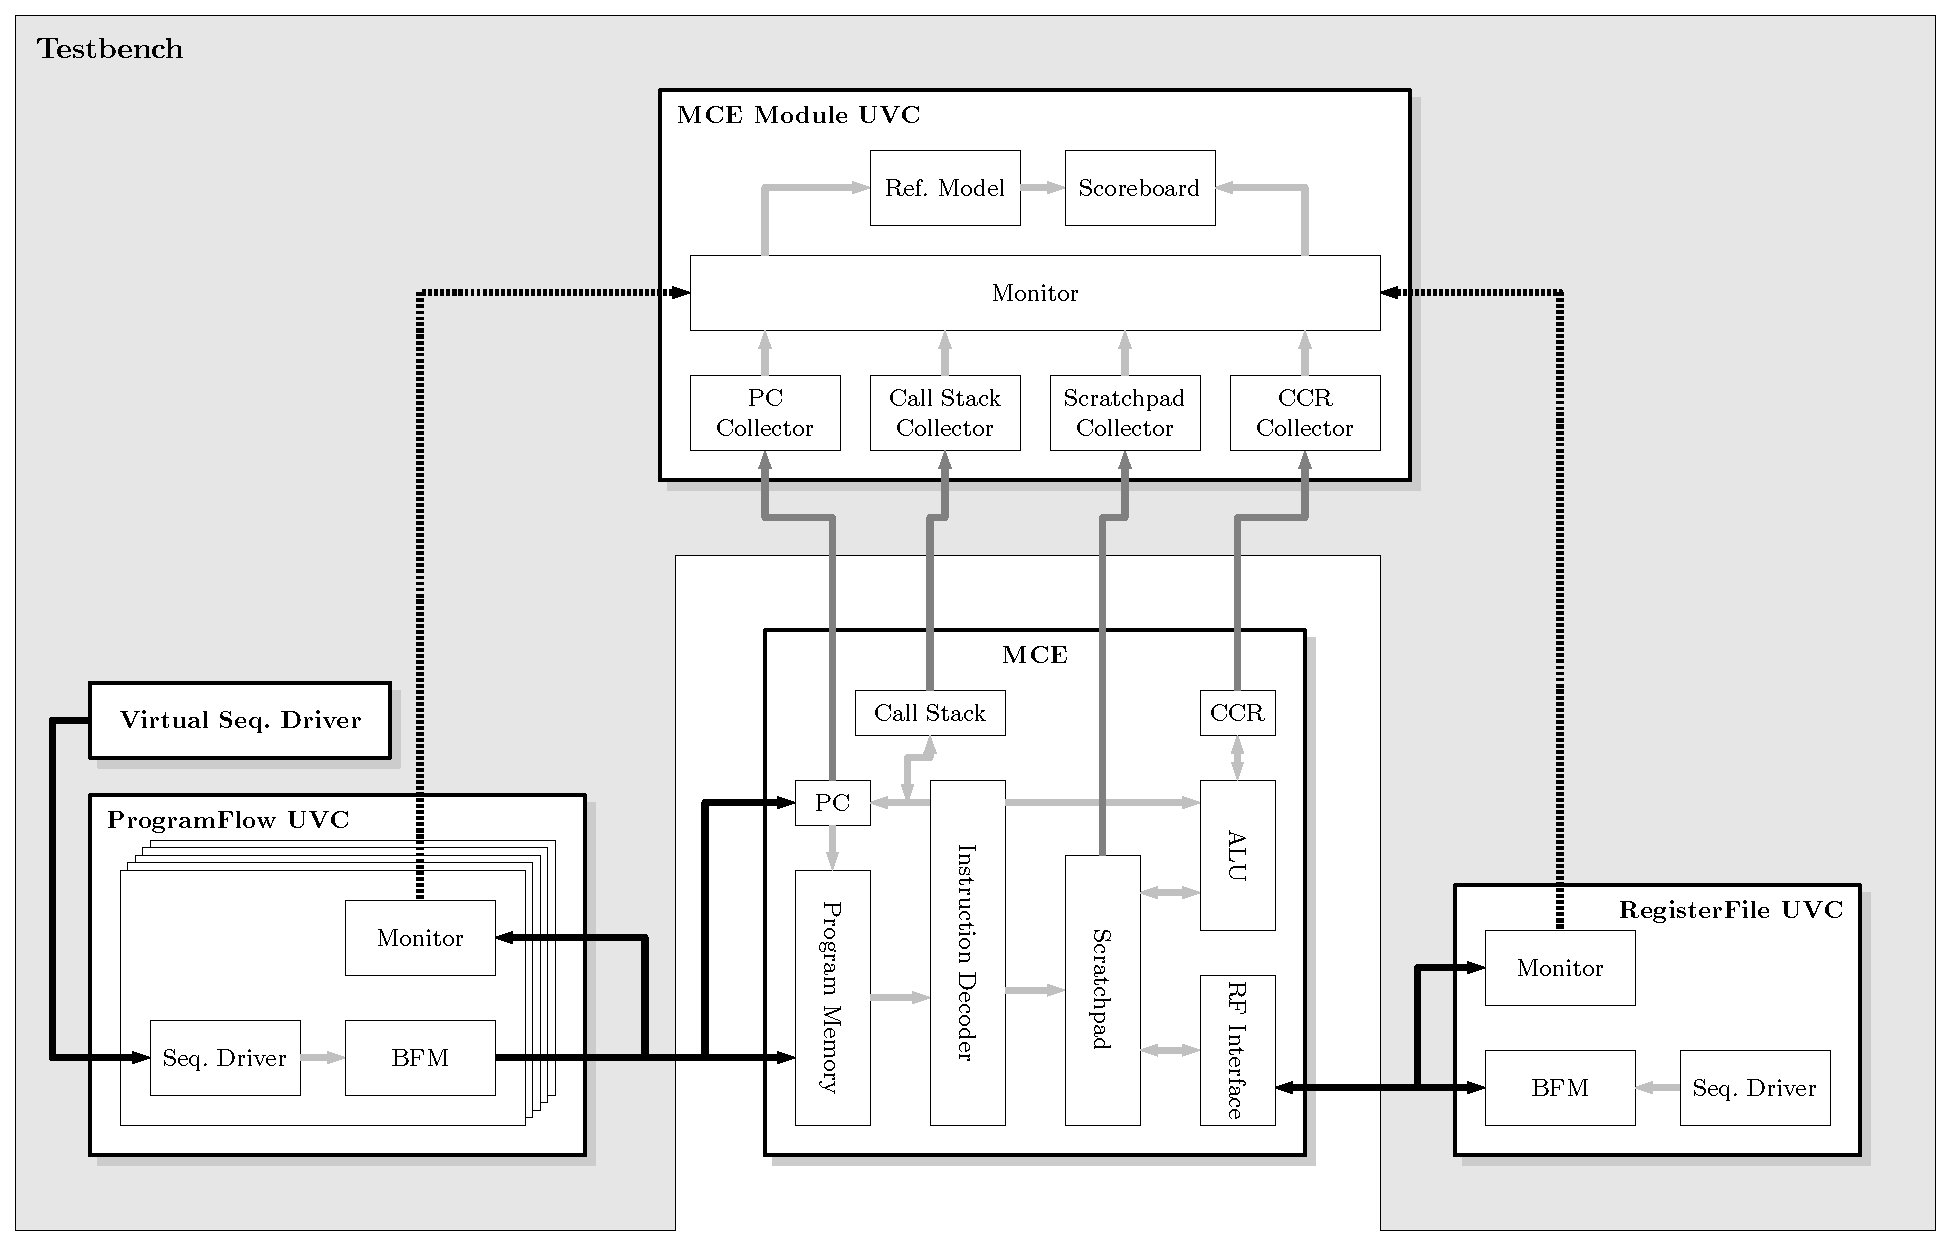
\includegraphics[width=1.0\textwidth,angle=0]{images/mce_tb}
 \caption{MCE Testbench}
\label{fig:mce_tb}
\end{figure}

\subsection{ProgramFlow Interface UVC}

The ProgramFlow interface UVC groups multiple interfaces of the MCE. 
It handles the instruction memory, external condition code bits, call stack overflow, start and done interface.
Thereby each interface has its own agent.
These agents are described in the following sections.

\subsubsection{Instruction Memory Agent}

\subsubsection{External Condition Code Bits Agent}

\subsubsection{Call Stack Overflow Agent}

\subsubsection{Start Agent}

\subsubsection{Done Agent}

\subsection{CSR Interface UVC}

The external memory interface is handled in the CSR interface UVC.
Its monitor samples the individual signals of the interface and creates an sequence item for each CSR access with the collected data.
This item is then sent to the module UVC via a TLM port.\\
When the MCE starts a transaction, the UVC has to respond to this request.
So if the monitor notices, that a transaction was started, it emits an event, causing the sequence driver to generate the response.
Since a memory access can take multiple clock cycles to complete, first a random number of up to 10 clock cycles is waited.
After that the UVC sends the access complete signal and additionally random data is returned for a read transaction.
Furthermore there is a chance, that the transaction is completed indicating an invalid address in addition to the access complete signal.

\subsection{MCE Module UVC}

The module UVC of the MCE has knowledge of the desired behavior of the DUT.
It uses a reference model to predicts the behavior of the engine for a given set of stimuli.
In the scoreboard the predicted results are then matched against the data received from the interface UVCs and its own collectors.
The structure of the module UVC is shown in figure~\ref{fig:module_uvc}.

\begin{figure}[htb]
 \centering
 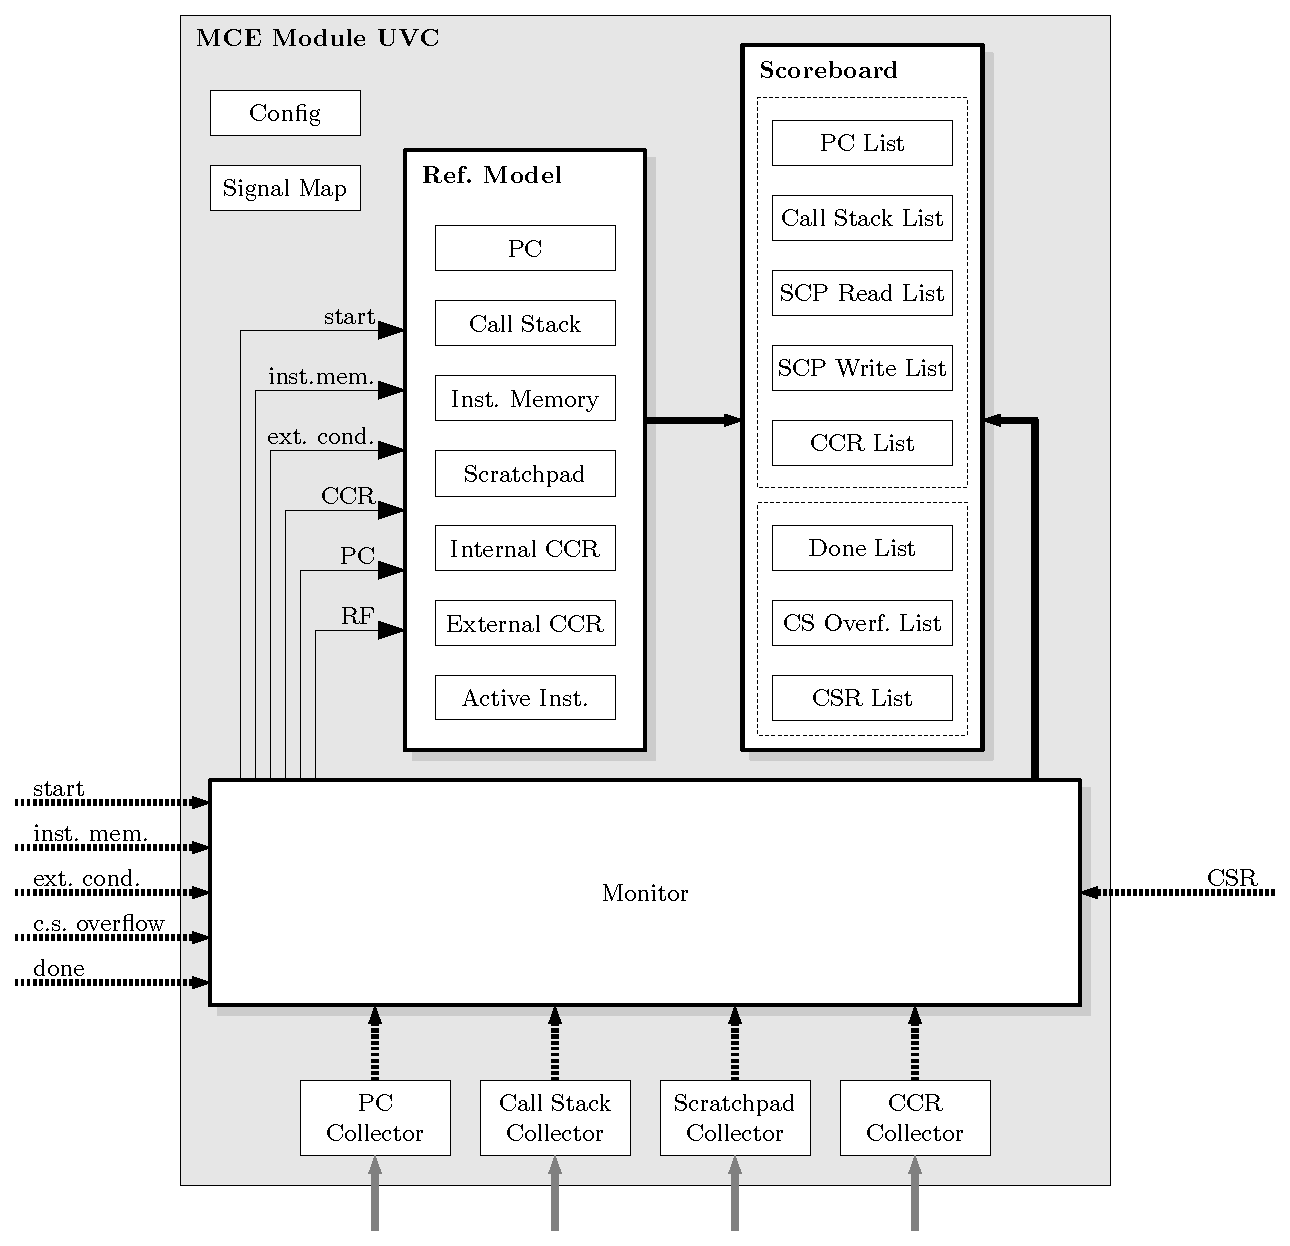
\includegraphics[width=1.0\textwidth,angle=0]{images/mce_module_uvc}
 %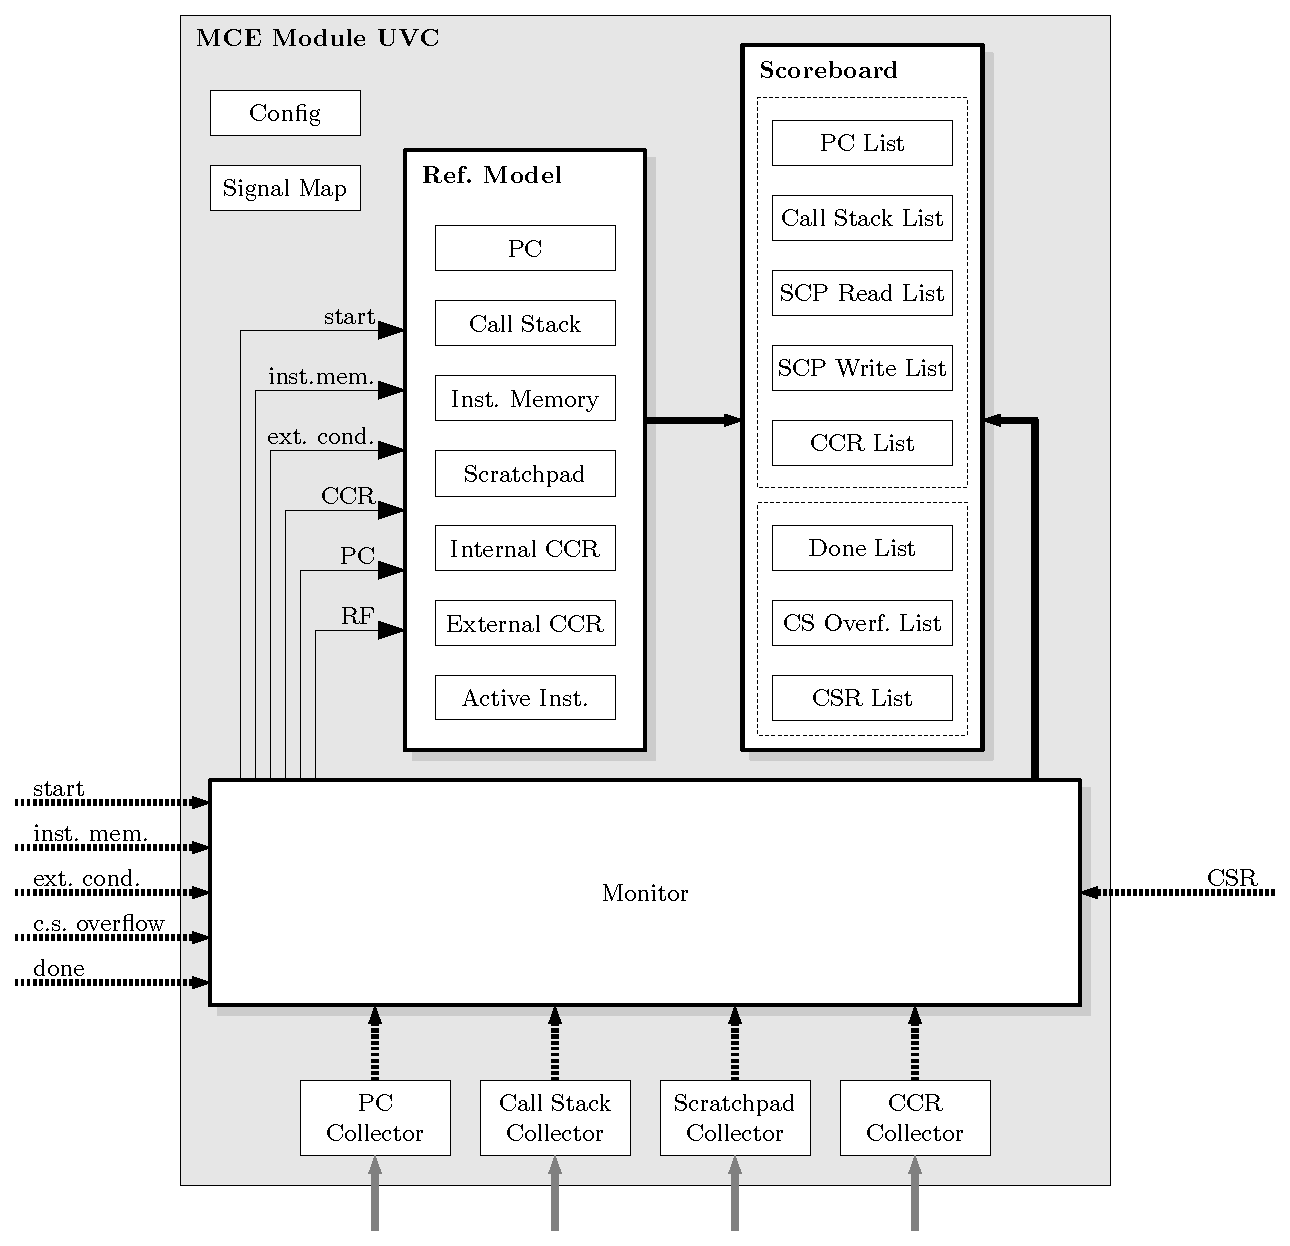
\includegraphics[scale=1.0]{images/mce_module_uvc}
 \caption{MCE Module UVC}
\label{fig:module_uvc}
\end{figure}

\subsubsection{Collectors}

Besides of the monitors of the interface UVCs, collectors are responsible for obtaining information about the DUT.
Where the monitors gather data from the interfaces of the design, the collectors receive their data from components inside of the MCE.
They are used to get a more precise insight on the current state of the DUT.
With these detailed information 
 

\paragraph{Program Counter Collector}

The program counter collector samples the current address of the PC.
It generates a new sequence item, whenever the PC is changed, while a program is running inside of the MCE.

\paragraph{Call Stack Collector}

The call stack collector observes the call stack of the design.
Whenever the index of the stack and therefore its size changes, a new transaction is created.
Thereby, a transaction contains the direction of the operation and the pushed or popped address, respectively.\\
In this process, the direction is derived from the change of the index.
If the index is incremented or an overflow occurs, a \emph{push} operation has been performed.
Whereas a decremented index indicates a \emph{pop} operation, except for an overflow.
Thereby, the exception of an call stack overflow occurs, if the call stack is currently empty and was full in the previous clock cycle.

\paragraph{Scratchpad Collector}

The scratchpad collector monitors the three ports of the scratchpad.
It generates sequence items for the read or write operations, respectively.
Thereby a sequence item contains the direction of the operation (read or write), the index of the port, the address of the accessed register as well as the read/written data.
Whereas the index of the write port is 0, of the first read port is 1 and of the second read port is 2.\\
When the normal program flow of the engine is disrupted by a conflicting external memory access, a single instruction can cause multiple consecutive write operations on the scratchpad. 
Since a memory access takes a unknown number of clock cycles to complete, it cannot be predicted, how many of these multiple write operations occur for an instruction.
However these multiple write operations do not change the state of the MCE.
Thus, it is sufficient to collect only the first operation of this series and ignore the following ones.
So no more than a single write operation is collected for a given instruction.\\
The MCE reads the scratchpad every clock cycle, while it is running a program.
Since reading the scratchpad does not influence its state, it is safe to do so.
Only the ALU determines, if the read data is required for the execution of an instruction.\\
Therefore the collector also takes the opcode of the instruction causing the read access into account.
So a transaction is only created, if the read access is realy necessary for the exection of the instruction.

\paragraph{Condition Code Register Collector}

The condition code register collector observes the write port of the CCR.
Whenever a condition code is written into it, a new sequence item is created.
It consists of the index identifying a specific register of the CCR and the condition code, which is written.\\
Since the CCR does not contain a read port (each bit can be accessed directly), only the write port is monitored.

\subsubsection{Monitor}

The monitor is the central component of the module UVC.
It forwards the transactions received from the interface UVCs and the collectors to the remaining components of the module UVC.
All the communication between the monitor and the interface UVCs as well as the collectors is handled via TLM ports.
Thereby, the connected components can easily be exchanged on demand.\\
Additionally to handling the communication between components, the monitor also collects coverage.
This occurs, whenever the monitor receives a transaction from the collectors.

\subsubsection{Scoreboard}

The scoreboard is an important component for the self-checking testbench.
It verifies the proper operation of the DUT.
Therefor, it contains a list of transactions for the components, which determine the state of the design.
In figure~\ref{fig:scoreboard} it is displayed, which lists are included in the scoreboard.
These lists are grouped according to where their items are collected.
The lists of the \emph{design internal} group are used for the internal signals monitored by the collectors of the module UVC.
Furthermore the lists of the \emph{design interfaces} group contain data gathered from the interface UVCs.

\begin{figure}[htb]
 \centering
 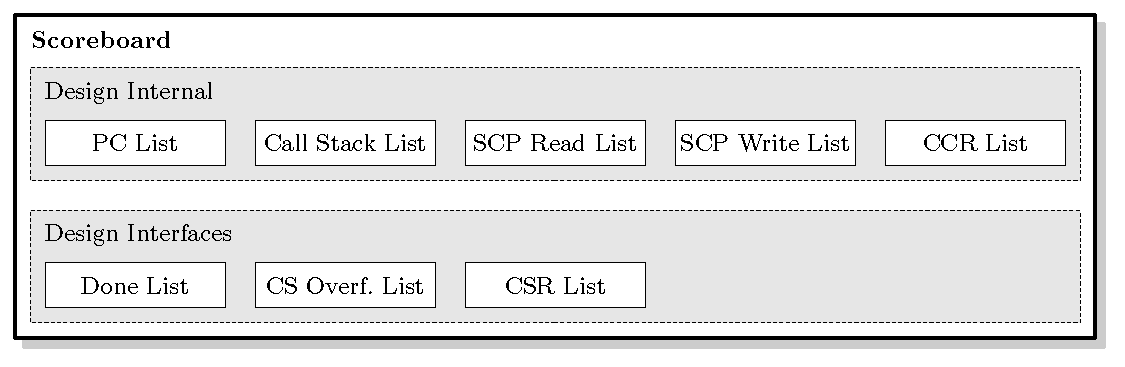
\includegraphics[width=1.0\textwidth,angle=0]{images/scoreboard}
 %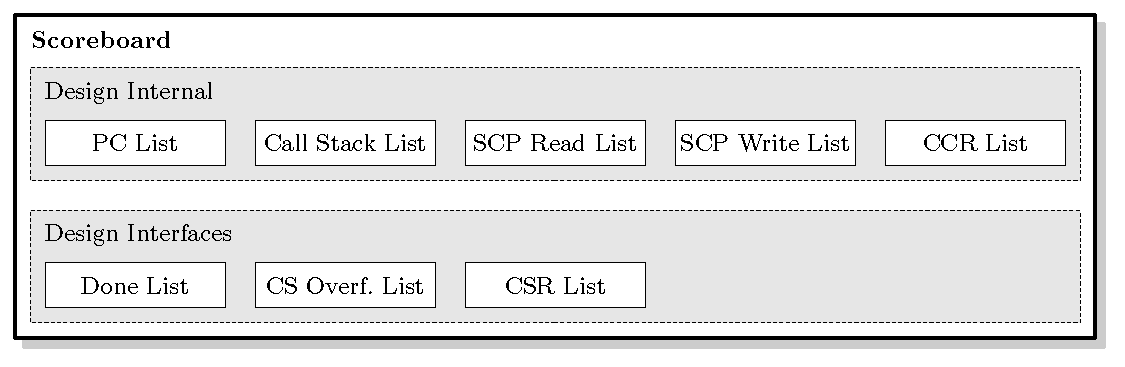
\includegraphics[scale=1.0]{images/scoreboard}
 \caption{Lists of the Scoreboard}
\label{fig:scoreboard}
\end{figure}

The procedure of checking within a general list is shown in figure~\ref{fig:scoreboard_flow}. 
Firstly, the predicted data from the reference model is added to the end of the list.
When a transaction is gathered by a collector or monitor of an interface UVC, it is send to the scoreboard.
After that, the received item is matched against the first item of the list.
If they match, both the reference model and the design produced equivalent data during their execution.
Otherwise either the testbench or the DUT contains a bug, which has to be fixed.\\
Needless to say, the list has to contain some items before any collected item can be matched.
Furthermore, at the end of a test run, all lists have to be empty.

\begin{figure}[htb]
 \centering
 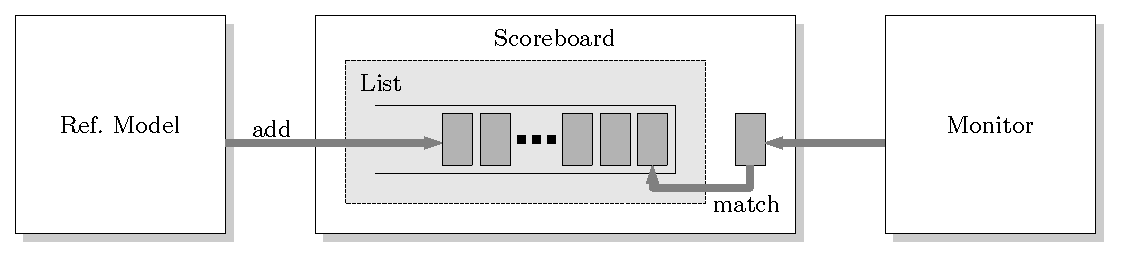
\includegraphics[width=1.0\textwidth,angle=0]{images/scoreboard_flow}
 %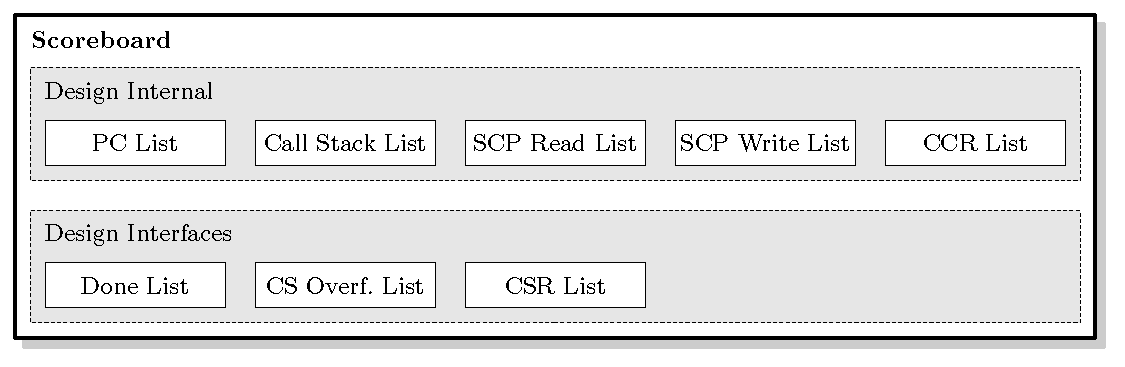
\includegraphics[scale=1.0]{images/scoreboard}
 \caption{Self-Checking within a General List}
\label{fig:scoreboard_flow}
\end{figure}

All lists except the scratchpad write list use this method.
Since the following instructions are executed while an external memory access is pending,
the order of the write operations on the scratchpad can change (see section~\ref{mem_access}).
However, the order of write operations on a specific register of the scratchpad is maintained.
Thus, collected scratchpad write operations are matched against the first item of the list with the same scratchpad address.
This is displayed in figure~\ref{fig:scoreboard_scp_write_flow}.

\begin{figure}[htb]
 \centering
 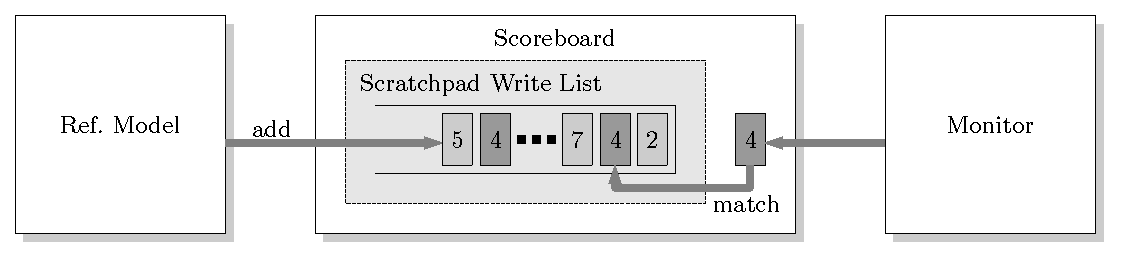
\includegraphics[width=1.0\textwidth,angle=0]{images/scoreboard_scp_write_flow}
 %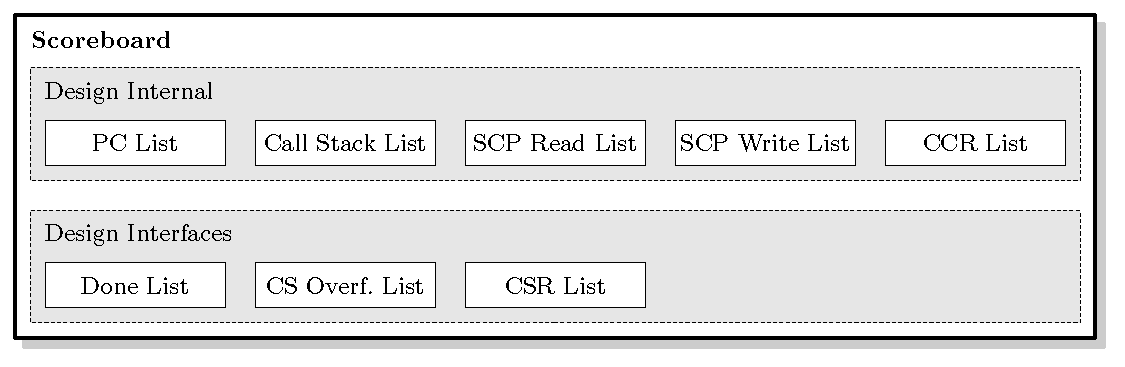
\includegraphics[scale=1.0]{images/scoreboard}
 \caption{Self-Checking within the Scratchpad Write List}
\label{fig:scoreboard_scp_write_flow}
\end{figure}


\subsubsection{Reference Model}

\paragraph{List of Active Instructions}

\paragraph{Instruction Execution Flow}

\paragraph{Stall Barrier}

\paragraph{Register File Read Transactions}

\paragraph{CCR Write Transactions}

\subsection{Virtual Sequence Driver}

\subsection{Test Library}